\documentclass[preview]{standalone}

\usepackage{caption, subcaption, tikz, amsmath}
\tikzset{>=latex}

\begin{document}

\tikzset{every picture/.style={line width=0.75pt}} %set default line width to 0.75pt        

\begin{figure}
\captionsetup[subfigure]{position=above}% reduce gap between picture and caption
\begin{subfigure}{0.26\textwidth}
\centering
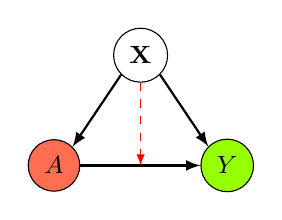
\begin{tikzpicture}
%\draw (1,1.5) circle (0.3cm)  node[anchor=center] {$X$};
%\draw[fill={rgb, 255:red, 255; green, 110; blue, 80 }, fill opacity=1] (0,0) circle (0.3cm) node[anchor=center] {$Z$};
%\draw[fill={rgb, 255:red, 150; green, 255; blue, 0 }, fill opacity=1] (2,0) circle (0.3cm) node[anchor=center] {$Y$};

\node[circle, draw=black] (X) at (1.1,1.4) {\small $\mathbf{X}$};
\node[circle, draw=black, fill={rgb, 255:red, 255; green, 110; blue, 80 }] (A) at (0,0) {\small $A$};
\node[circle, draw=black, fill={rgb, 255:red, 150; green, 255; blue, 0 }] (Y) at (2.2,0) {\small $Y$};

\draw[thick, ->] (X.south east) -- (Y.north west);
\draw[thick, ->] (X.south west) -- (A.north east);
\draw[thick, ->] (A.east) -- (Y.west);
\draw[thin, dashed, ->, red] (X.south) -- (1.1, 0);
\end{tikzpicture}
\end{subfigure} % no space between subfigures
\begin{subfigure}{0.26\textwidth}
\centering
\small
\begin{align*}
    & \mathbf{X} = f_X (\varepsilon_X) \\
    & A = f_A (\mathbf{X}, \varepsilon_A) \\
    & Y = f_Y (\mathbf{X}, A) + \varepsilon_Y
\end{align*}
\vspace{-0.01cm}
\end{subfigure} \hspace{0.2cm} % no space between subfigures
\end{figure}
\end{document}